\documentclass[12pt,a4paper]{article}
\usepackage{newtxtext,newtxmath}
\usepackage[utf8]{inputenc}
\usepackage[T1]{fontenc}
\usepackage[margin=2.5cm]{geometry}
\usepackage[
backend=biber,
style=apa
]{biblatex}

\addbibresource{referencias.bib}
\usepackage{xcolor}
\usepackage{setspace}
\usepackage{csquotes}
\usepackage{titlesec}
\titleformat{\section}
{\Huge\bfseries\color{azulnoche}}
{\thesection}
{1em}
{}

\titleformat{\subsection}
{\Large\bfseries\color{azulnoche}}
{\thesubsection}
{1em}
{}

\titleformat{\subsubsection}
{\large\bfseries\color{azulnoche}}
{\thesubsubsection}
{1em}
{}
\usepackage{colortbl}
\usepackage{graphicx}
\usepackage{caption}
\captionsetup{compatibility=false}
\usepackage{booktabs}
\usepackage{tocloft}
\usepackage[spanish]{babel}
\usepackage{hyperref}
\usepackage{float}
\usepackage{tabularx}
\usepackage{array}
\hypersetup{
    colorlinks=true,
    linkcolor=azulnoche,
    urlcolor=azulnoche
}

\setlength{\parindent}{1.5em}
\onehalfspacing
\setlength{\cftbeforesecskip}{6pt}
\renewcommand{\contentsname}{Índice}

\definecolor{azulnoche}{RGB}{0,40,90}
\definecolor{celesteclaro}{RGB}{224,240,255}
\definecolor{grisclaro}{RGB}{245,245,245}
\definecolor{darkgreen}{rgb}{0.533, 0.486, 0.184}
\definecolor{golden}{RGB}{197,160,89}
\definecolor{goldford}{RGB}{143,113,54}
\definecolor{rojo}{RGB}{166,25,46}


\renewcommand{\cftsecfont}{\color{azulnoche}\bfseries\itshape}
\renewcommand{\cftsubsecfont}{\color{azulnoche}\bfseries\itshape}
\renewcommand{\cftsubsubsecfont}{\color{azulnoche}\bfseries\itshape}

\renewcommand{\cftsecpagefont}{\color{azulnoche}}
\renewcommand{\cftsubsecpagefont}{\color{azulnoche}}
\renewcommand{\cftsubsubsecpagefont}{\color{azulnoche}}

\renewcommand{\cftsecpresnum}{\color{azulnoche}}
\renewcommand{\cftsubsecpresnum}{\color{azulnoche}}
\renewcommand{\cftsubsubsecpresnum}{\color{azulnoche}}

\renewcommand{\cftsecaftersnum}{\color{azulnoche}}
\renewcommand{\cftsubsecaftersnum}{\color{azulnoche}}
\renewcommand{\cftsubsubsecaftersnum}{\color{azulnoche}}

\begin{document}

\begin{titlepage}
\centering
{\color{golden}\bfseries\large UNIVERSIDAD NACIONAL MAYOR DE SAN MARCOS}\\
\vspace{0.1cm}
{\color{golden}\large\textbf{Universidad del Perú, Decana de América}}\\
\vspace{0.5cm}

\includegraphics[width=0.35\textwidth]{oso.png}\\
\vspace{0.5cm}
{\color{goldford}\scshape\Large Facultad de Ingeniería de Sistemas e Informática\\}
{\color{goldford}\scshape\large Escuela Profesional de Ingeniería de Sistemas\\}
\vspace{0.56cm}
\color{rojo}\hrule height 0.3mm\vspace{0.5cm}
{\color{rojo}\Large\bfseries MONOGRAFÍA: AWS\vspace{0.56cm}}\\
\color{rojo}\hrule height 0.3mm\vspace{0.5cm}
{\color{rojo}\Large\textbf{Curso:}}\\
\vspace{0.1cm}
{\color{goldford}\Large Introducción a la Computación}\\
\vspace{0.5cm}
{\color{rojo}\Large\textbf{Docente:}}\\
\vspace{0.1cm}
{\color{goldford}\Large Gelber Christian Uscuchagua Flores}\\
\vspace{0.5cm}
{\color{rojo}\Large\textbf{Integrantes:}}\\
\vspace{0.1cm}
{\color{goldford}\Large Mamani Huahualuque, Airton Abedal}\\
{\color{goldford}\Large Mundo Dominguez, Adair Andre}\\
{\color{goldford}\Large Cruz Mora, Angel Josue}\\
{\color{goldford}\Large Flores Villalba, Gianella Alexandra}\\
\vspace{0.5cm}
{\color{rojo}\Large\textbf{Grupo:}}\\
\vspace{0.1cm}
{\color{goldford}\Large Gitverso - UscuchaguaLovers}\\
\vspace{1.4cm}
{\color{goldford}\Large\textbf{Lima, 12 de Julio del 2026}}\\
\end{titlepage}

% ==============================
% ÍNDICE
% ==============================
\tableofcontents
\newpage

% =========================================================================
% 1. INTRODUCCIÓN
% =========================================================================
\section{Introducción}

La infraestructura tecnológica ha evolucionado de forma acelerada en las últimas décadas, debido a la migración de sistemas locales hacia entornos virtuales remotos.

Este avance se refleja principalmente en la computación en la nube, un modelo que ha redefinido el almacenamiento, procesamiento y distribución de datos en las organizaciones actuales.

\subsection{Contextualización}

El procesamiento de datos pasó de un enfoque tradicional basado en la compra de hardware físico local (infraestructura \textit{On-Premise}) a un entorno flexible y accesible a través de Internet. Este cambio reestructuró la gestión financiera de las empresas al sustituir las inversiones de capital fijas y de alta depreciación (CapEx) por un esquema de gastos operativos variables basados en el consumo real (OpEx) \parencite{mell2011}. 

En este mercado, Amazon Web Services (AWS) destaca como el proveedor con mayor adopción a nivel global. Desde su lanzamiento comercial en 2006, AWS fue pionero en ofrecer servicios de infraestructura elástica y actualmente mantiene cerca del 32\% de la cuota del mercado mundial de nube pública \parencite{gartner2024, statista2025}. Su arquitectura soporta desde plataformas de entretenimiento masivo y banca transaccional, hasta entornos de desarrollo para Inteligencia Artificial Generativa y sistemas gubernamentales.

\subsection{Justificación}

El estudio de AWS es clave para la ingeniería y las ciencias de la computación debido a su adopción masiva en la industria actual. Comprender su funcionamiento permite evaluar conceptos esenciales como la abstracción de hardware, la virtualización avanzada y la alta disponibilidad en entornos de producción. 

No obstante, la centralización de gran parte de la infraestructura de Internet en una sola corporación privada plantea riesgos técnicos y operativos que requieren una evaluación detallada. Este trabajo se justifica al ofrecer una perspectiva completa: analiza las soluciones de ingeniería que hacen de AWS una plataforma tolerante a fallos y, al mismo tiempo, examina de forma crítica las implicaciones sobre la dependencia del proveedor (\textit{vendor lock-in}), la seguridad de los datos y la competencia en el mercado tecnológico actual \parencite{armbrust2010}.

\subsection{Objetivos del estudio}

\subsubsection{Objetivo General}
Analizar de manera integral el ecosistema de Amazon Web Services (AWS), evaluando sus fundamentos teóricos, su arquitectura de infraestructura y el impacto de su dominio en el mercado tecnológico actual.

\subsubsection{Objetivos Específicos}
\begin{itemize}
    \item Analizar la evolución histórica de AWS y su relación con los modelos de servicio (IaaS, PaaS, SaaS) y de despliegue según los estándares del NIST.
    \item Detallar la infraestructura física y los mecanismos de virtualización de AWS, explicando el funcionamiento de Regiones, Zonas de Disponibilidad y el Sistema AWS Nitro.
    \item Evaluar los avances tecnológicos de la plataforma en el desarrollo de silicio propio y herramientas orientadas a la Inteligencia Artificial Generativa.
    \item Examinar las principales limitaciones del ecosistema, incluyendo el análisis de costos, las caídas de red y los desafíos de regulación antimonopolio.
\end{itemize}

\subsection{Metodología del estudio}

Esta investigación se desarrolla bajo un enfoque cualitativo, de diseño no experimental y nivel descriptivo. La metodología se basa en la revisión bibliográfica de fuentes técnicas y académicas. Las fuentes revisadas incluyen estándares internacionales del Instituto Nacional de Estándares y Tecnología (NIST), reportes de mercado (Gartner, Statista), artículos de ciencias de la computación y la documentación oficial de AWS. La información se clasificó y sintetizó para desarrollar el marco teórico y el análisis crítico de las secciones posteriores.



\section{Capítulo I}

Este capítulo sirve como base teórica del trabajo. El objetivo es entender cómo nació, cambió y se consolidó el modelo de computación en la nube como el motor de la infraestructura digital del siglo XXI. Para ello, se examina en primer lugar el trayecto evolutivo de Amazon.com, Inc., analizando los factores operativos e internos que impulsaron su metamorfosis de comercio minorista a líder tecnológico global con el nacimiento de AWS. Posteriormente, se abordan las bases normativas e internacionales del paradigma \textit{cloud} según los estándares del NIST, para finalmente catalogar de forma analítica los diversos modelos de despliegue y de servicio que articulan el desarrollo de software contemporáneo. Con este recorrido, se establecen los cimientos conceptuales necesarios para el desglose técnico y crítico de las secciones posteriores.

\subsection{Contexto Histórico: }

Para comprender el origen de la computación en la nube moderna, es necesario analizar la transformación estructural de Amazon.com, Inc. Fundada en 1994 por Jeffrey Bezos como una librería en línea, la compañía experimentó una expansión masiva y acelerada durante su primera década de existence. Hacia el año 2000, la plataforma de comercio electrónico de Amazon se había convertido en un ecosistema altamente complejo, .pero su infraestructura tecnológica tenía un diseño monolítico que le impedía crecer y escalar de forma eficiente \parencite{varia2014}. 

Los equipos de ingeniería de la empresa invertían un porcentaje desproporcionado de su tiempo en tareas de aprovisionamiento de hardware, configuración de bases de datos y diseño de redes personalizadas para cada nuevo proyecto o función que se deseaba lanzar al mercado. La infraestructura física de la compañía operaba en silos aislados, lo que provocaba que los recursos computacionales se duplicaran de forma ineficiente y que los ciclos de desarrollo de software se extendieran durante semanas o meses. 

Ante esta problemática, la dirección técnica de Amazon, bajo la guía de figuras clave como el actual director ejecutivo Andy Jassy y el director de tecnología (CTO) Werner Vogels, inició una reestructuración radical de sus sistemas. Alrededor del año 2002, se emitió un mandato corporativo interno que obligaba a todos los equipos de desarrollo a desacoplar sus aplicaciones y a exponer sus datos y funcionalidades exclusivamente a través de Interfaces de Programación de Aplicaciones (APIs) estrictamente estandarizadas e independientes del hardware subyacente.

Esta transformación hacia una Arquitectura Orientada a Servicios (SOA) interna permitió que las capacidades de cómputo, red y almacenamiento de Amazon se abstrajeran y unificaran. El equipo directivo descubrió que, al construir esta plataforma común y estandarizada para resolver sus propios problemas de optimización y crecimiento minorista, habían diseñado un conjunto de servicios de infraestructura altamente eficientes que poseían un valor comercial intrínseco masivo si se ofrecían a desarrolladores y empresas externas \parencite{awsWhatIs}.
\subsection{El nacimiento de AWS}
La formalización de esta infraestructura como un modelo de negocio independiente dio origen a Amazon Web Services (AWS), cuya plataforma fue presentada oficialmente al mercado global en marzo de 2006. El hito fundacional de la computación en la nube moderna se consolidó con el lanzamiento de su primer servicio comercial enfocado en el almacenamiento de objetos: \textit{Amazon Simple Storage Service} (S3). En agosto del mismo año, AWS expandió su catálogo con la introducción de \textit{Amazon Elastic Compute Cloud} (EC2), un servicio que permitía a los usuarios alquilar capacidad de procesamiento virtualizada por horas o minutos \parencite{awsWhatIs}.

El impacto de este lanzamiento fue disruptivo en el ámbito de las ciencias de la computación y la administración de tecnologías de la información. Por primera vez en la historia de la informática, las organizaciones de cualquier tamaño podían omitir la adquisición física de servidores y conmutadores de red, sustituyéndolos por llamadas programáticas a APIs remotas conectadas a internet \parencite{armbrust2010}.

A lo largo de las dos décadas siguientes, la cronología evolutiva de AWS se caracterizó por una diversificación constante de sus servicios e innovaciones de arquitectura, los cuales se resumen en la siguiente línea de tiempo:

\vspace{0.3cm}
\begin{table}[H]
\centering
\caption{Cronología Evolutiva de Amazon Web Services (2006–2026)}
\label{tab:cronologia_aws}
\begin{tabular}{ l p{5cm} p{6.5cm} }
\toprule
\textbf{Año} & \textbf{Hito Tecnológico / Servicio} & \textbf{Impacto en el Paradigma del Cloud} \\
\midrule
\textbf{2006} & Lanzamiento de Amazon S3 y EC2. & Fundación de la nube pública comercial moderna. \\
\textbf{2009} & Introducción de Amazon VPC. & Permitió el aislamiento lógico y la adopción empresarial. \\
\textbf{2012} & Lanzamiento de Amazon DynamoDB. & Democratización de bases de datos NoSQL de baja latencia. \\
\textbf{2014} & Presentación de AWS Lambda. & Inauguración oficial de la computación sin servidores (\textit{Serverless}). \\
\textbf{2017} & Lanzamiento de Amazon SageMaker. & Masificación del entrenamiento y despliegue de \textit{Machine Learning}. \\
\textbf{2023--2026} & Despliegue de Amazon Bedrock. & Consolidación de la infraestructura para IA Generativa a escala global. \\
\bottomrule
\end{tabular}
\end{table}
\vspace{0.3cm}
\subsection{Conceptos fundamentales del Cloud Computing}
Para darle a esta investigación un tono más académico, el análisis de la computación en la nube debe fundamentarse en el marco teórico establecido por el Instituto Nacional de Estándares y Tecnología (NIST) de los Estados Unidos. En su informe especial 800-145, \textcite{mell2011} definen formalmente el \textit{Cloud Computing} como un modelo tecnológico que facilita el acceso ubiquo, adaptativo y bajo demanda a un conjunto compartido de recursos de computación configurables (redes, servidores, almacenamiento, aplicaciones y servicios) que pueden ser aprovisionados y liberados de manera inmediata con un mínimo esfuerzo de gestión por parte del usuario.

\vspace{0.2cm}
\begin{quote}
\small
\textit{\enquote{La computación en la nube es un modelo que permite el acceso ubicuo, conveniente y bajo demanda a un fondo compartido de recursos informáticos configurables (por ejemplo, redes, servidores, almacenamiento, aplicaciones y servicios) que pueden aprovisionarse y liberarse rápidamente con un mínimo esfuerzo de gestión o interacción con el proveedor del servicio.}} \parencite[p.~2]{mell2011}.
\end{quote}
\vspace{0.2cm}

De acuerdo con este estándar internacional, el modelo de computación en la nube se sostiene de forma obligatoria sobre cinco características esenciales detalladas en la siguiente tabla:

\vspace{0.3cm}
\begin{table}[H]
\centering
\caption{Matriz de Características Esenciales del Cloud Computing (NIST)}
\label{tab:nist_caracteristicas}
\begin{tabular}{ p{4.5cm} p{8cm} }
\toprule
\textbf{Característica NIST} & \textbf{Principio Operativo Clave} \\
\midrule
Autoservicio bajo demanda & Aprovisionamiento automatizado sin intervención humana del proveedor. \\
Acceso amplio a la red & Disponibilidad multiplataforma (móvil, web, servidores) vía HTTP/HTTPS. \\
Asignación común de recursos & Infraestructura física compartida dinámicamente (\textit{Multi-tenancy}). \\
Elasticidad rápida & Escalabilidad horizontal y vertical automática según la demanda de tráfico. \\
Servicio medido & Facturación transparente basada en el consumo real (\textit{Pay-as-you-go}). \\
\bottomrule
\end{tabular}
\end{table}
\vspace{0.3cm}
\subsection{Modelos de Despliegue de la Nube: Pública, Privada e Híbrida}

La implementación estratégica de la computación en la nube varía significativamente en función de la propiedad, la exclusividad del hardware y la ubicación geográfica de los centros de datos físicos. El NIST clasifica estas configuraciones en tres modelos de despliegue principales: Nube Pública, Nube Privada y Nube Híbrida \parencite{mell2011}. Para fines analíticos, sus diferencias estructurales se examinan bajo criterios de propiedad, modelo financiero y casos de uso en la Tabla \ref{tab:modelos_despliegue}.

\vspace{0.3cm}
\begin{table}[H]
\centering
\caption{Diferencias Estructurales entre los Modelos de Despliegue}
\label{tab:modelos_despliegue}
\begin{tabular}{ p{2.8cm} p{3.4cm} p{3.4cm} p{3.4cm} }
\toprule
\textbf{Criterio} & \textbf{Nube Pública} & \textbf{Nube Privada} & \textbf{Nube Híbrida} \\
\midrule
\textbf{Propiedad} & Proveedor (AWS). & Una sola organización. & Entorno mixto interconectado. \\
\textbf{Esquema} & Costos operativos (OpEx). & Inversión de capital (CapEx). & Mixto (Local + elástico). \\
\textbf{Multitenancia} & Compartido lógicamente. & Aislado físicamente. & Mixto según sensibilidad. \\
\textbf{Caso de Uso} & \textit{Startups}, apps web, IA. & Sector defensa, banca, salud. & Corporaciones en transición. \\
\bottomrule
\end{tabular}
\end{table}
\vspace{0.3cm}

\subsection{Modelos de Servicio: Infraestructura (IaaS), Plataforma (PaaS) y Software (SaaS)}

La abstracción de componentes en la computación en la nube divide el catálogo técnico en tres categorías conceptuales o modelos de servicio primarios. Estos modelos delimitan con precisión el nivel de control y la división de responsabilidades operativas entre el proveedor de nube y el cliente final \parencite{subashini2011}. Por último para cerrar el capítulo, la Tabla \ref{tab:modelos_servicio} contrasta la matriz de responsabilidades e incluye los ejemplos de aplicación directa en el catálogo de AWS.

\vspace{0.3cm}
\begin{table}[H]
\centering
\caption{Tabla Comparativa de los Modelos de Servicio en la Nube}
\label{tab:modelos_servicio}
\begin{tabular}{ p{3.2cm} p{3.4cm} p{3.4cm} p{3.4cm} }
\toprule
\textbf{Criterio} & \textbf{IaaS (Infraestructura)} & \textbf{PaaS (Plataforma)} & \textbf{SaaS (Software)} \\
\midrule
\textbf{Abstracción} & Bajo (Control de hardware virtual). & Medio (Entornos de ejecución). & Alto (Aplicación lista para el usuario). \\
\textbf{Cliente} & S.O., datos, \textit{firewalls} y código. & Datos y código de la aplicación. & Ninguna (Solo gestiona usuarios). \\
\textbf{AWS} & Servidores, red e hipervisor. & Parches S.O. y base de datos. & Toda la pila de software e interfaces. \\
\textbf{Ejemplo AWS} & Amazon EC2, Amazon EBS \parencite{varia2014}. & AWS Elastic Beanstalk, RDS. & Amazon WorkSpaces, AWS Wickr. \\
\bottomrule
\end{tabular}
\end{table}
\vspace{0.3cm}

\section{Capítulo II}
La infraestructura de Amazon Web Services (AWS) constituye uno de los ecosistemas de computación en la nube más grandes del mundo. Su arquitectura está diseñada para proporcionar alta disponibilidad, escalabilidad, seguridad y tolerancia a fallos mediante una red global de centros de datos distribuidos estratégicamente. En este capítulo se describen los principales componentes de la infraestructura de AWS, la ingeniería de sus centros de datos, la tecnología de virtualización utilizada, los principales servicios que ofrece y el modelo de responsabilidad compartida en materia de seguridad.

\subsection{Topología de la Infraestructura Mundial: Regiones y AZs}

La infraestructura mundial de Amazon Web Services (AWS) está conformada por una red global de centros de datos distribuidos estratégicamente en distintos continentes. Esta infraestructura permite que las aplicaciones y servicios operen con baja latencia, alta disponibilidad y redundancia, garantizando la continuidad del servicio incluso ante fallas de hardware o desastres naturales\parencite{awsInfrastructure}.

La arquitectura global de AWS se basa en diferentes componentes, entre ellos las Regiones (\textit{Regions}), las Zonas de Disponibilidad (\textit{Availability Zones}), las Local Zones y las Edge Locations. Cada uno cumple una función específica para optimizar el rendimiento, la disponibilidad y la cercanía con los usuarios finales.

El diseño distribuido de AWS permite que los recursos puedan replicarse entre diferentes zonas y regiones, facilitando la recuperación ante desastres y el balanceo de carga.

\begin{figure}[H]
\centering
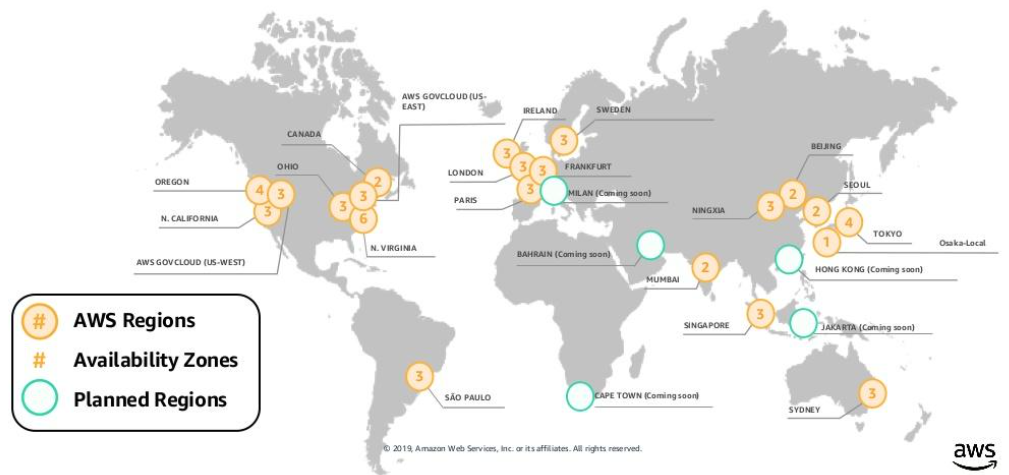
\includegraphics[width=0.95\textwidth]{regiones.png}
\caption{Infraestructura mundial de AWS: regiones y zonas de disponibilidad.}
\label{fig:regiones}
\end{figure}

\begin{table}[H]
\centering
\caption{Componentes de la infraestructura mundial de AWS}
\begin{tabularx}{\textwidth}{lXX}
\toprule
\textbf{Componente} & \textbf{Descripción} & \textbf{Función}\\
\midrule
Región (Region) & Área geográfica donde AWS posee centros de datos. & Alojar servicios y recursos.\\

Zona de Disponibilidad (AZ) & Uno o varios centros de datos independientes dentro de una región. & Garantizar alta disponibilidad.\\

Local Zone & Extensión de una región ubicada cerca de grandes ciudades. & Reducir la latencia.\\

Edge Location & Centros de distribución utilizados por CloudFront y Route 53. & Entrega rápida de contenido.\\

Backbone Global & Red privada de fibra óptica de AWS. & Comunicación segura entre regiones.\\
\bottomrule
\end{tabularx}
\end{table}

\subsection{Ingeniería de los Centros de Datos: Redundancia y Climatización}

Los centros de datos de AWS están diseñados siguiendo estrictos estándares internacionales de seguridad, disponibilidad y eficiencia energética\parencite{awsDatacenters}. Cada instalación incorpora sistemas redundantes de energía eléctrica, refrigeración, conectividad y almacenamiento para minimizar el riesgo de interrupciones del servicio.

La infraestructura física emplea controles de acceso biométricos, monitoreo permanente mediante cámaras de vigilancia y personal especializado disponible las 24 horas del día. Además, AWS implementa sistemas automáticos de detección y extinción de incendios, así como mecanismos de respaldo energético mediante UPS y generadores eléctricos.

Otro aspecto importante es la eficiencia energética. AWS optimiza continuamente el consumo de energía mediante tecnologías avanzadas de refrigeración y el uso creciente de fuentes de energía renovables \parencite{awsSustainability}.

\begin{figure}[H]
\centering
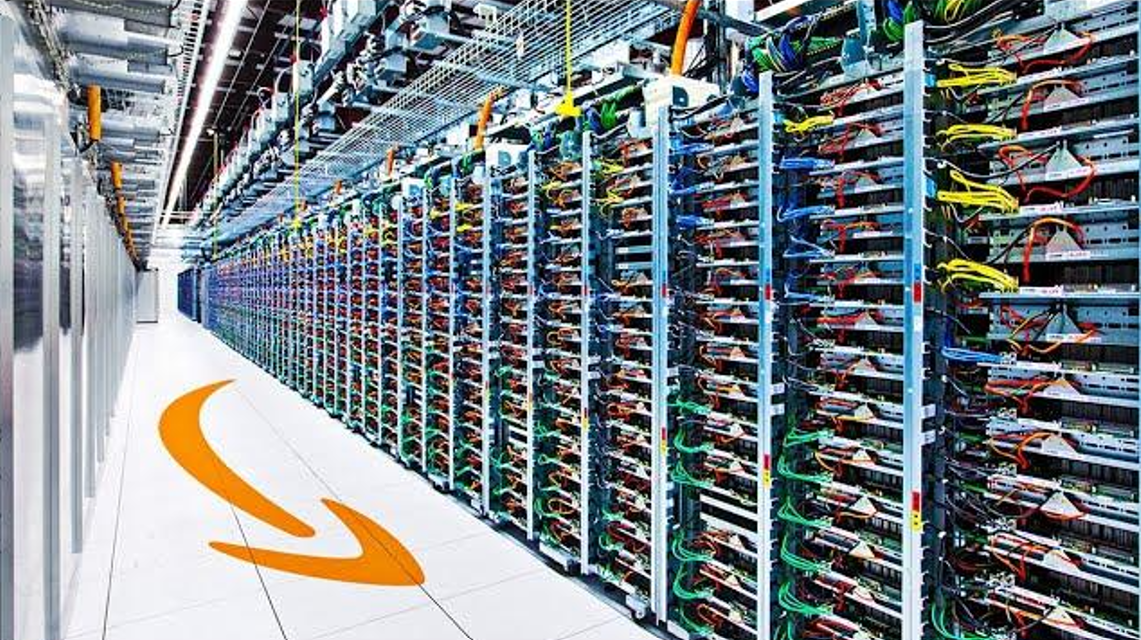
\includegraphics[width=0.90\textwidth]{datacc.png}
\caption{Centro de datos de Amazon Web Services.}
\label{fig:datacenter}
\end{figure}

\begin{table}[H]
\centering
\caption{Características de los centros de datos de AWS}
\begin{tabularx}{\textwidth}{lX}
\toprule
\textbf{Característica} & \textbf{Descripción}\\
\midrule
Seguridad física & Acceso biométrico, vigilancia permanente y control de ingreso.\\

Redundancia eléctrica & UPS, generadores y múltiples fuentes de alimentación.\\

Refrigeración & Sistemas inteligentes para mantener temperaturas óptimas.\\

Conectividad & Múltiples enlaces de red de alta velocidad.\\

Monitoreo & Supervisión continua de infraestructura y servicios.\\

Escalabilidad & Posibilidad de ampliar recursos sin interrupciones.\\
\bottomrule
\end{tabularx}
\end{table}

\subsection{Virtualización Avanzada: Sistema AWS nitro}

La virtualización constituye una de las tecnologías fundamentales sobre las que se basa Amazon Web Services\parencite{awsNitro}. Esta técnica permite ejecutar múltiples máquinas virtuales sobre un mismo servidor físico, optimizando el uso de los recursos computacionales y reduciendo los costos operativos.

AWS utiliza principalmente el sistema AWS Nitro, una plataforma que integra hardware y software especializado para mejorar el rendimiento, la seguridad y el aislamiento entre instancias. Gracias a esta arquitectura, los usuarios pueden crear servidores virtuales en cuestión de minutos, escalarlos automáticamente y administrar cargas de trabajo de diferentes tamaños\parencite{awsNitro}.

La virtualización también facilita la automatización de recursos, la recuperación ante fallos y el despliegue rápido de aplicaciones.

\begin{table}[H]
\centering
\caption{Tipos de virtualización utilizados por AWS}
\begin{tabularx}{\textwidth}{lXX}
\toprule
\textbf{Tipo} & \textbf{Descripción} & \textbf{Servicio}\\
\midrule
Virtualización de servidores & Divide un servidor físico en varias máquinas virtuales. & Amazon EC2\\

Virtualización de almacenamiento & Agrupa varios discos físicos como una sola unidad lógica. & Amazon EBS\\

Virtualización de redes & Redes definidas por software. & Amazon VPC\\

Virtualización de escritorios & Escritorios virtuales administrados. & Amazon WorkSpaces\\
\bottomrule
\end{tabularx}
\end{table}

\subsection{Catálogo de Servicios Pilares}

Amazon Web Services ofrece más de doscientos servicios en la nube. Entre ellos destacan tres pilares fundamentales para el funcionamiento de cualquier infraestructura tecnológica: cómputo, almacenamiento y bases de datos.

\subsubsection{Cómputo (Amazon EC2, AWS Lambda)}

Los servicios de cómputo proporcionan capacidad de procesamiento para ejecutar aplicaciones, sitios web, servicios empresariales y algoritmos de inteligencia artificial. AWS permite aprovisionar recursos bajo demanda y pagar únicamente por el tiempo utilizado\parencite{amazonEC2}.

Estos servicios pueden escalar automáticamente según la demanda, permitiendo responder de manera eficiente a incrementos en el tráfico de usuarios.

\begin{figure}[H]
\centering
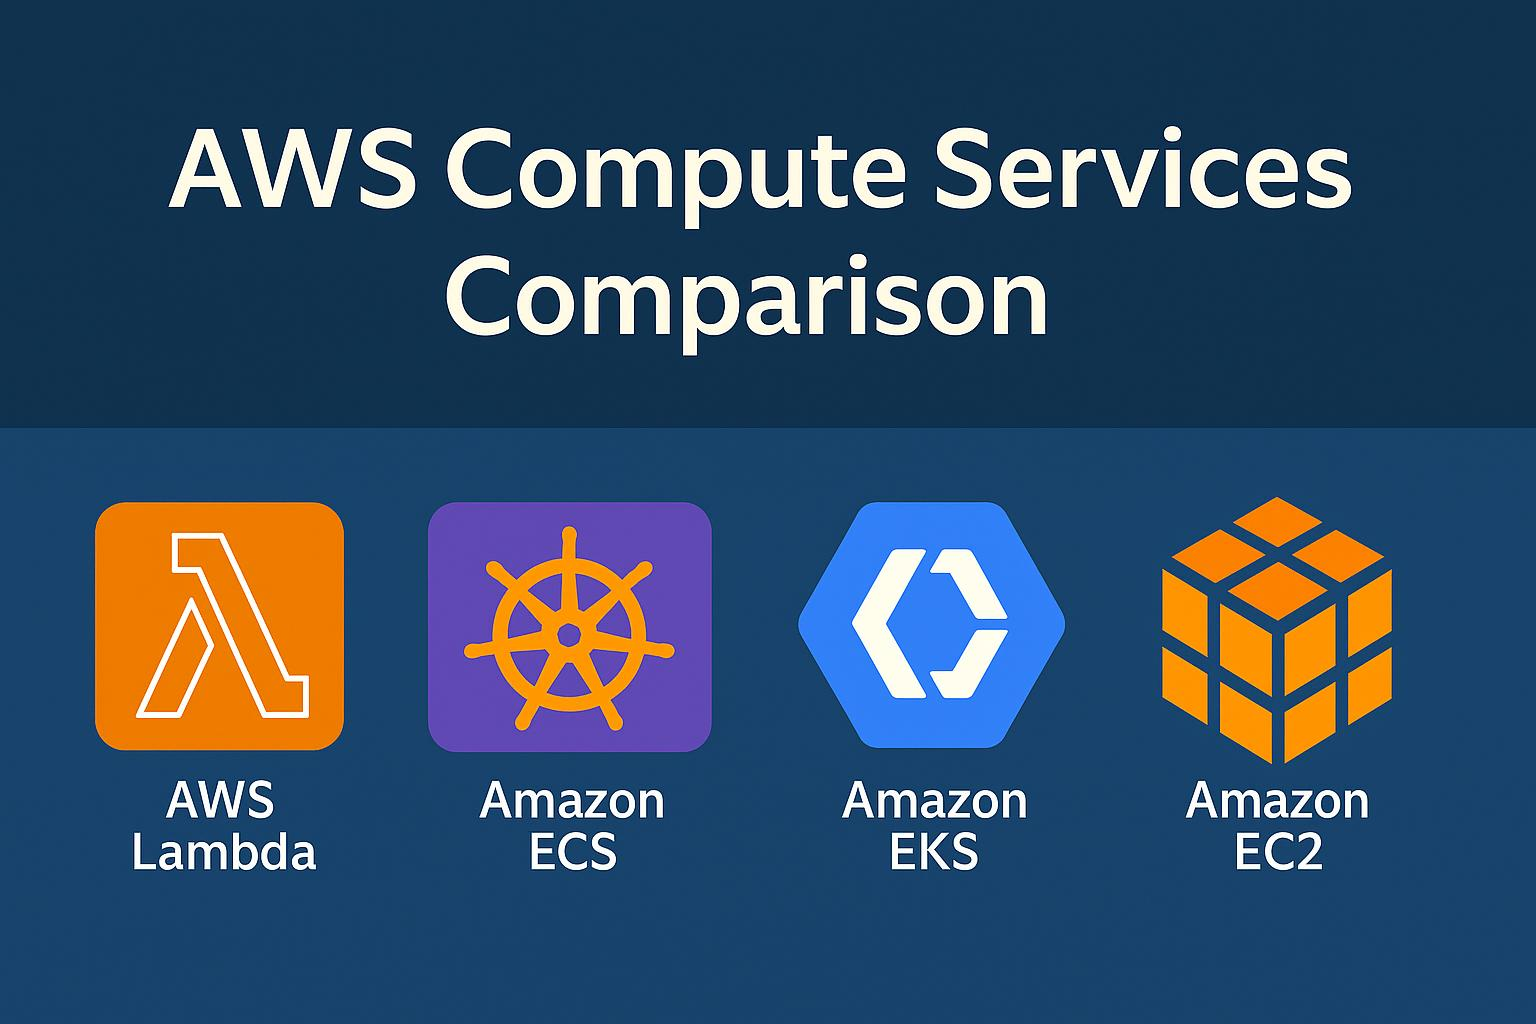
\includegraphics[width=0.60\textwidth]{computo.jpg}
\caption{Principales servicios de cómputo de AWS.}
\label{fig:computo}
\end{figure}

\begin{table}[H]
\centering
\caption{Servicios de cómputo de AWS}
\begin{tabularx}{\textwidth}{lX}
\toprule
\textbf{Servicio} & \textbf{Función}\\
\midrule
Amazon EC2 & Máquinas virtuales bajo demanda.\\

AWS Lambda & Ejecución de funciones sin administrar servidores.\\

Elastic Beanstalk & Implementación automática de aplicaciones.\\

Amazon ECS & Administración de contenedores Docker.\\

Amazon EKS & Kubernetes administrado.\\

Amazon Lightsail & Infraestructura simplificada para pequeñas aplicaciones.\\
\bottomrule
\end{tabularx}
\end{table}

\subsubsection{Almacenamiento (Amazon S3, EBS, Glacier)}

Los servicios de almacenamiento permiten guardar información de manera segura, escalable y altamente disponible. AWS ofrece diferentes alternativas según las necesidades de cada aplicación, incluyendo almacenamiento por objetos, bloques y sistemas de archivos compartidos\parencite{amazonS3}.

\begin{figure}[H]
\centering
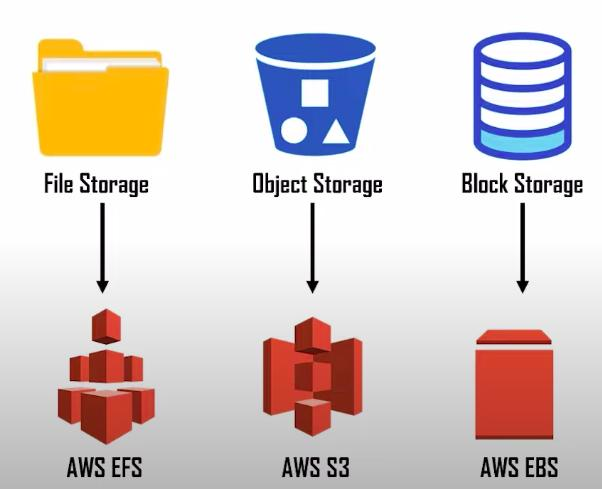
\includegraphics[width=0.65\textwidth]{almacenamiento.jpg}
\caption{Tipos de almacenamiento disponibles en AWS.}
\label{fig:almacenamiento}
\end{figure}

\begin{table}[H]
\centering
\caption{Servicios de almacenamiento de AWS}
\begin{tabularx}{\textwidth}{lXX}
\toprule
\textbf{Servicio} & \textbf{Tipo} & \textbf{Uso principal}\\
\midrule
Amazon S3 & Objetos & Archivos, imágenes y copias de seguridad.\\

Amazon EBS & Bloques & Discos virtuales para EC2.\\

Amazon EFS & Archivos & Sistemas Linux compartidos.\\

AWS Backup & Respaldo & Copias de seguridad automáticas.\\

Amazon FSx & Archivos & Sistemas Windows y Lustre.\\
\bottomrule
\end{tabularx}
\end{table}

\subsubsection{Bases de Datos (RDS, DynamoDB, Aurora)}

AWS proporciona servicios administrados para bases de datos relacionales y NoSQL, permitiendo almacenar grandes volúmenes de información con alta disponibilidad y escalabilidad. La administración automática reduce la carga operativa de los administradores de bases de datos\parencite{amazonRDS}.

\begin{figure}[H]
\centering
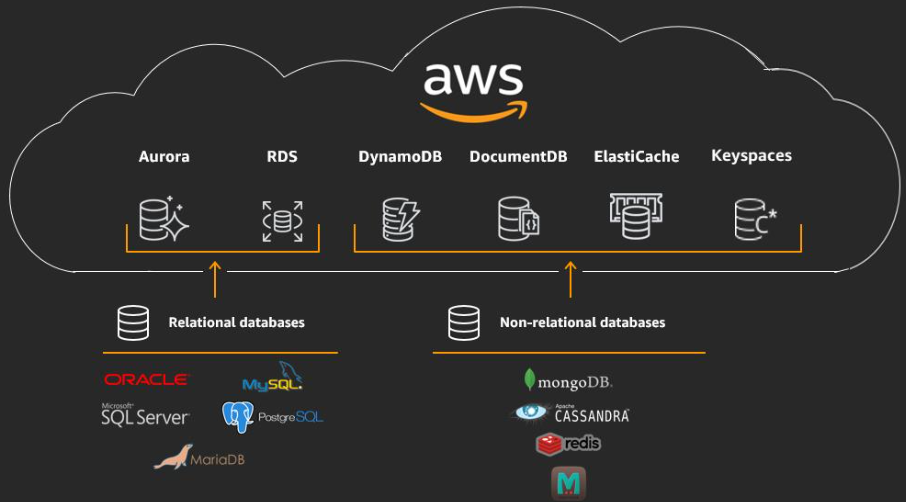
\includegraphics[width=0.75\textwidth]{basedato.png}
\caption{Servicios administrados de bases de datos en AWS.}
\label{fig:basedatos}
\end{figure}

\begin{table}[H]
\centering
\caption{Servicios de bases de datos de AWS}
\begin{tabularx}{\textwidth}{lXX}
\toprule
\textbf{Servicio} & \textbf{Tipo} & \textbf{Aplicación}\\
\midrule
Amazon RDS & Relacional & Aplicaciones empresariales.\\

Amazon Aurora & Relacional & Alto rendimiento compatible con MySQL y PostgreSQL.\\

Amazon DynamoDB & NoSQL & Aplicaciones web y móviles.\\

Amazon Redshift & Data Warehouse & Inteligencia de negocios.\\

Amazon ElastiCache & Caché & Aceleración de aplicaciones.\\
\bottomrule
\end{tabularx}
\end{table}

\subsection{Modelo de la Responsabilidad Compartida en Seguridad y Redes}

Uno de los principios fundamentales de AWS es el modelo de responsabilidad compartida, el cual define claramente las responsabilidades que corresponden al proveedor de servicios en la nube y aquellas que deben ser asumidas por el cliente.

AWS es responsable de proteger la infraestructura física que soporta los servicios en la nube, incluyendo los centros de datos, el hardware, la red física y el software de virtualización. Por otro lado, el cliente es responsable de proteger sus datos, administrar los accesos de usuarios, configurar adecuadamente los servicios utilizados y mantener actualizados sus sistemas operativos cuando corresponda.

Este modelo permite que ambas partes colaboren para garantizar un entorno seguro y confiable.

\begin{table}[H]
\centering
\caption{Modelo de responsabilidad compartida}
\begin{tabularx}{\textwidth}{XX}
\toprule
\textbf{Responsabilidad de AWS} & \textbf{Responsabilidad del Cliente}\\
\midrule
Protección de centros de datos & Protección de los datos\\

Infraestructura física & Administración de usuarios\\

Hardware y almacenamiento & Configuración de servicios\\

Red física & Actualización del sistema operativo\\

Hipervisor y plataforma & Gestión de permisos y políticas IAM\\

Disponibilidad global & Cifrado de la información\\
\bottomrule
\end{tabularx}
\end{table}

\section{Capítulo III}

\subsection{AWS como Motor de la Economía Digital}

AWS revolucionó los modelos de servicio en la nube al popularizar comercialmente el concepto \textbf{XaaS} (\textit{Anything as a Service}), que en pocas palabras expresa que \textbf{cualquier recurso tecnológico puede ser ofrecido y consumido como un servicio}. Esta filosofía nació con un objetivo claro: resolver los históricos problemas de \textbf{alto costo y alta complejidad} que implicaban gestionar y configurar infraestructuras TI tradicionales.

Gracias a su amplio portafolio de servicios, AWS ha democratizado el acceso a la tecnología. En este sentido, ha sido un habilitador clave para las \textbf{startups}, modelos de negocio que suelen operar con presupuestos reducidos y necesitan salir al mercado con rapidez. Con AWS, estas empresas ya no se ven limitadas por su infraestructura TI, ya que pueden desplegar y escalar aplicaciones en minutos sin realizar fuertes inversiones iniciales.

Además, AWS ha roto una barrera histórica: \textbf{pone al alcance de cualquier emprendedor tecnologías que, inicialmente, solo estaban disponibles para las gigantes del mercado}, como inteligencia artificial, machine learning, bases de datos distribuidas o computación de alto rendimiento. De este modo, nivela el campo de juego y fomenta la innovación sin importar el tamaño de la organización.

AWS se ha convertido en un pilar indispensable de la economía digital al ser la plataforma elegida por los gigantes tecnológicos que mueven el mundo: \textbf{Netflix} (con más de 100.000 instancias), \textbf{Twitch}, \textbf{LinkedIn}, \textbf{Facebook}, \textbf{Twitter}, además de entidades como la NASA Su adopción masiva, más del 90\% del Fortune 100 utiliza su red de socios, y los ahorros operativos que genera (como el 50\% de reducción logrado por General Electric o Unilever) demuestran que AWS no solo ofrece infraestructura, sino que \textbf{acelera la innovación, reduce costes y nivela el campo de juego}, permitiendo que tanto startups como corporaciones globales compitan con la misma potencia tecnológica en la era digital.

\subsection{Innovación en Silicio Propio}

La estrategia de hardware de AWS ha evolucionado de un modelo de compra a una integración vertical diseñada para romper la dependencia de terceros y optimizar el rendimiento por dólar invertido. Históricamente, NVIDIA ha consolidado un monopolio casi absoluto en el mercado de aceleradores informáticos, controlando aproximadamente cuatro de cada cinco unidades distribuidas globalmente, lo que ha generado una dependencia que encarece los costos de entrenamiento de modelos a gran escala.

En respuesta a este escenario, AWS ha comenzado a comercializar sus chips \textbf{Trainium}, posicionándolos como una alternativa de alto rendimiento específicamente diseñada para el entrenamiento de modelos de Inteligencia Artificial. A diferencia de las soluciones de propósito general, Trainium optimiza los ciclos de cómputo en redes neuronales y reduce la latencia de transferencia de datos entre los núcleos de cómputo y la memoria de alta fidelidad. De este modo, AWS no solo compite en precio, sino también en \textbf{eficiencia energética}, tal como ya lo hace con los procesadores \textbf{Graviton}.

Con esta estrategia, la compañía no solo reduce costes operativos para sus clientes, sino que también refuerza su posición como proveedor integral, desafiando el dominio de NVIDIA y ofreciendo una alternativa viable que combina rendimiento, eficiencia y soberanía tecnológica dentro de su ecosistema.

\subsection{Proyectos Disruptivos y Planes Futuros}

La estrategia de innovación de AWS se orienta a acercar la computación a quien la usa, rompiendo con la idea de depender solo de grandes centros de datos. En lugar de esperar a que los usuarios lleguen a una nube central, AWS propone reducir la latencia y abrir nuevas posibilidades explorando tecnologías emergentes como la computación cuántica. A continuación describo tres iniciativas que encajan con esa visión.

\begin{itemize}
\item \textbf{AWS Local Zones:} La idea es llevar la infraestructura de AWS más cerca de las ciudades, industrias y equipos de TI, colocándola en ubicaciones periféricas cercanas a los usuarios. De este modo, operaciones que requieren respuestas en milisegundos, como juegos, streaming de video en alta definición y ciertas aplicaciones financieras, pueden funcionar de forma más fluida sin depender únicamente de las regiones centrales muy alejadas geográficamente.

\item \textbf{AWS Wavelength:} Pensado para redes 5G, Wavelength inserta los servicios de AWS directamente en la periferia de las redes de los operadores de telecomunicaciones. En lugar de que los datos tengan que viajar hasta un centro de datos lejano y volver, el procesamiento ocurre junto a la infraestructura de la red, en el borde. Esto reduce enormemente la latencia, a menos de 10 milisegundos en muchos casos, y facilita usos como la inferencia de IA en el borde, juegos en la nube, realidad aumentada y diagnóstico médico remoto.

\item \textbf{Amazon Braket:} Braket es la entrada de AWS a la computación cuántica. Es un servicio totalmente gestionado que da acceso a diferentes tipos de procesadores cuánticos y a simuladores clásicos para pruebas. Su propósito es democratizar la experimentación con algoritmos cuánticos, permitiendo a investigadores y desarrolladores explorar soluciones a problemas complejos de optimización, modelado molecular y criptografía, sin la necesidad de invertir en una infraestructura cuántica propia.
\end{itemize}

\subsection{AWS y la IA Generativa}

La Inteligencia AI Generativa es, en esencia, una rama de la IA que no solo analiza o clasifica datos, sino que crea contenido nuevo. Si la IA tradicional se encarga de decirte si una imagen contiene un gato o un perro, la IA generativa puede dibujar un gato que nunca antes ha existido, escribir un poema con tu estilo o componer una melodía. Esta capacidad se obtiene entrenando algoritmos de aprendizaje profundo con volúmenes masivos de datos —textos, imágenes, códigos o audio— para que aprendan patrones, estructuras y relaciones complejas. Una vez entrenados, estos modelos, denominados modelos fundacionales (entre ellos destacan los Large Language Models o LLM), generan respuestas originales y contextualmente coherentes gracias a arquitecturas de Transformadores, que procesan secuencias de datos con gran eficiencia. Su valor real no está solo en interpretar el mundo, sino en recrearlo, lo que abre posibilidades antes impensables en creatividad, automatización y toma de decisiones.

La relación entre AWS y la IA Generativa es profundamente simbiótica, ya que esta tecnología exige potencia de cómputo, capacidad de almacenamiento y velocidad de red que solo una infraestructura de hiperescala como la de AWS puede ofrecer. AWS actúa como el habilitador industrial de esta revolución tecnológica sobre tres pilares fundamentales: la democratización, que permite a empresas de cualquier tamaño acceder a modelos fundacionales sin construir infraestructura desde cero; la soberanía de datos, que garantiza la integración segura de modelos públicos con datos privados y propietarios, crucial en entornos regulados; y la escalabilidad, que permite ejecutar inferencias —el uso de los modelos para generar respuestas— a millones de usuarios simultáneamente, manteniendo una baja latencia esencial para aplicaciones en tiempo real.

Para hacer concreta esta visión, AWS ha reconfigurado su oferta y desarrollado cuatro hitos clave que reducen drásticamente las barreras de entrada a la IA Generativa. El primero es Amazon Bedrock, un servicio gestionado que ofrece, mediante una única API, acceso a modelos fundacionales de alto rendimiento, tanto propios como Amazon Titan, como de terceros incluyendo Anthropic, Meta y Mistral, lo que permite a los ingenieros seleccionar el modelo más adecuado según costo, precisión y latencia sin complicaciones operativas. En segundo lugar, AWS ha desarrollado chips especializados: Trainium para entrenamiento e Inferentia para inferencia, que atacan directamente el problema de los costos energéticos y económicos de ejecutar modelos de lenguaje complejos, ofreciendo un rendimiento optimizado por dólar invertido. Luego viene SageMaker JumpStart, un centro de despliegue donde los desarrolladores pueden encontrar, probar y desplegar modelos preentrenados con un solo clic, automatizando la configuración del entorno de MLOps y acelerando considerablemente el time-to-market. Finalmente, AWS ha facilitado la arquitectura de sistemas RAG (Retrieval-Augmented Generation) dentro de su ecosistema, permitiendo que los modelos de IA consulten bases de datos como Amazon Aurora o el Vector Engine para OpenSearch en tiempo real Esta capacidad es fundamental porque mitiga el problema de las alucinaciones de los modelos.


\section{Capítulo IV}
En los capítulos anteriores se analizó el origen de Amazon Web Services (AWS), su evolución tecnológica y el papel que desempeña como uno de los principales proveedores de infraestructura en la nube. Sin embargo, el liderazgo alcanzado por la compañía también ha generado una serie de cuestionamientos relacionados con la concentración del mercado, la dependencia tecnológica, la seguridad operativa y las políticas regulatorias que actualmente comienzan a desarrollarse en distintos países.

El presente capítulo aborda estos aspectos desde una perspectiva crítica. Para ello, se examina la posición dominante de AWS dentro del mercado mundial de servicios en la nube, los riesgos asociados al uso de infraestructuras altamente centralizadas, las consecuencias arquitectónicas y financieras derivadas del denominado \textit{vendor lock-in}, el impacto que han tenido algunas interrupciones masivas de servicio y las principales iniciativas regulatorias impulsadas por distintos organismos internacionales.


\subsection{Análisis de Cuota de Mercado Global y Concentración del Poder Tecnológico}
La cuota de mercado constituye uno de los principales indicadores utilizados para medir el grado de participación que posee una empresa dentro de un determinado sector económico. En el caso de la computación en la nube, este indicador refleja el porcentaje de ingresos generados por cada proveedor respecto al total del mercado mundial de servicios de infraestructura (\textit{Infrastructure as a Service}, IaaS) y plataforma (\textit{Platform as a Service}, PaaS).

Amazon Web Services logró consolidar esta posición gracias a su ventaja de haber sido el primer proveedor en ofrecer servicios comerciales de nube pública desde el año 2006. Este hecho le permitió construir una infraestructura global antes que sus competidores y desarrollar economías de escala que todavía representan una importante barrera de entrada para nuevas empresas.

De acuerdo con el informe publicado por Synergy Research Group, durante el último trimestre analizado el mercado mundial de infraestructura en la nube superó los 119 mil millones de dólares en ingresos trimestrales y alcanzó más de 419 mil millones de dólares acumulados durante el año. Dentro de este escenario, AWS continúa ocupando el primer lugar con una participación aproximada del 28\% del mercado mundial, seguido por Microsoft Azure con un 21\% y Google Cloud Platform con un 14\%. El porcentaje restante corresponde a otros proveedores como Oracle Cloud, IBM Cloud, Alibaba Cloud y diversas empresas especializadas.\parencite{synergy2026}

\begin{figure}[H]
\centering
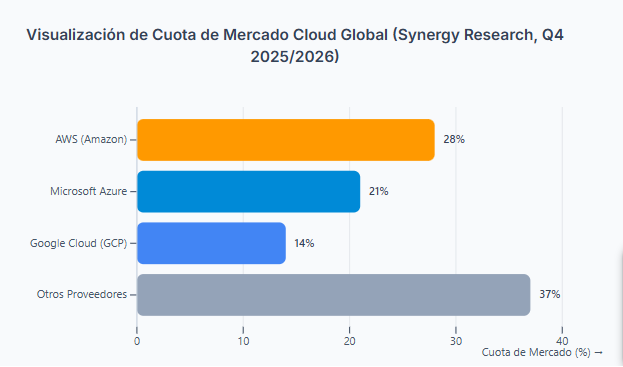
\includegraphics[width=0.85\textwidth]{Distribucion.png}
\caption{Distribución de la cuota de mercado mundial de los principales proveedores de servicios en la nube. Adaptado de Synergy Research Group.}
\label{fig:cuota_mercado}
\end{figure}

Más allá de representar una ventaja comercial, esta distribución evidencia un elevado nivel de concentración tecnológica. Actualmente, los tres principales proveedores de nube pública controlan aproximadamente el 68\% del mercado global, configurando una estructura cercana a un oligopolio tecnológico.\parencite{synergy2026}

Esta concentración se explica principalmente por dos factores. El primero corresponde al fenómeno conocido como \textit{data gravity}, según el cual las organizaciones tienden a mantener sus aplicaciones y bases de datos dentro del mismo proveedor debido al elevado costo económico y operativo que implica trasladar grandes volúmenes de información hacia otra plataforma. El segundo factor está relacionado con el crecimiento acelerado de la Inteligencia Artificial Generativa (GenAI), cuya infraestructura requiere inversiones multimillonarias en centros de datos, aceleradores gráficos (GPU) y redes de alta velocidad, recursos que actualmente solo pueden ser financiados por un reducido grupo de compañías tecnológicas.\parencite{synergy2026}

Como consecuencia, gran parte de la infraestructura digital utilizada por empresas, instituciones públicas y organizaciones privadas depende actualmente de un número muy limitado de proveedores. Esta situación incrementa el poder de negociación de estas compañías y reduce las posibilidades de migrar hacia plataformas alternativas sin asumir importantes costos económicos y técnicos.\parencite{cma2025}


\subsection{Riesgos Arquitectónicos y Financieros}
El crecimiento de la computación en la nube ha permitido que organizaciones de todos los tamaños reduzcan costos de infraestructura y aumenten la disponibilidad de sus servicios. Sin embargo, este modelo también ha dado lugar a nuevos desafíos relacionados con la dependencia tecnológica y la administración financiera de los recursos en la nube. Entre ellos destacan el fenómeno conocido como \textit{vendor lock-in} y la creciente complejidad de los modelos de facturación utilizados por los grandes proveedores.\parencite{cma2025}

El término \textit{vendor lock-in} hace referencia a la situación en la que una organización desarrolla una dependencia significativa hacia un único proveedor de servicios, dificultando la migración hacia otras plataformas sin asumir elevados costos económicos o técnicos. En el caso de AWS, este fenómeno surge debido a la utilización de numerosos servicios propietarios que, aunque ofrecen un alto nivel de integración y rendimiento, reducen considerablemente la portabilidad de las aplicaciones.\parencite{cma2025}

Servicios como Amazon DynamoDB, AWS Lambda, Amazon Cognito o Amazon S3 poseen interfaces de programación (API) diseñadas específicamente para el ecosistema de AWS. Como consecuencia, cuando una empresa desarrolla sus aplicaciones utilizando estas tecnologías, trasladarlas posteriormente a plataformas como Microsoft Azure o Google Cloud implica modificar parte importante del software, realizar nuevas pruebas e incluso rediseñar componentes completos de la arquitectura.\parencite{cma2025}

Otro aspecto ampliamente discutido corresponde a las denominadas tarifas de salida de datos (\textit{egress fees}). Mientras que AWS permite transferir información hacia sus propios centros de datos sin costo adicional, la extracción de grandes volúmenes de datos hacia infraestructuras externas suele generar cargos económicos importantes. Según el informe publicado por la Competition and Markets Authority (CMA), estas tarifas constituyen una de las principales barreras para la adopción de estrategias de nube híbrida o multi-nube, ya que incrementan significativamente el costo de migración entre proveedores.\parencite{cma2025}

A esta situación se suma la complejidad del modelo de facturación implementado por los proveedores de nube pública. El esquema de pago por uso (\textit{pay-as-you-go}) ofrece flexibilidad para contratar únicamente los recursos consumidos; sin embargo, las facturas suelen incluir cientos o miles de registros asociados al procesamiento, almacenamiento, transferencia de datos, solicitudes realizadas y otros servicios especializados. Esta característica dificulta el control del gasto, especialmente en organizaciones con una gran cantidad de aplicaciones desplegadas.

Como respuesta a esta problemática ha surgido la disciplina conocida como \textit{FinOps}, cuyo objetivo consiste en optimizar el uso de los recursos en la nube mediante el análisis permanente de los costos, la planificación presupuestaria y la identificación de servicios infrautilizados o innecesarios. Actualmente, numerosas empresas incorporan equipos especializados en FinOps para mejorar la eficiencia financiera de sus infraestructuras tecnológicas.

La Tabla \ref{tab:barreras_aws} resume los principales riesgos arquitectónicos y financieros identificados por la Competition and Markets Authority (CMA) durante su investigación sobre el mercado de servicios en la nube.

\begin{table}[H]
\centering
\caption{Barreras arquitectónicas y financieras identificadas en AWS. Adaptado de CMA (2025).}
\label{tab:barreras_aws}

\begin{tabular}{p{3.2cm}p{3.8cm}p{4.6cm}p{3.8cm}}
\toprule
\textbf{Dimensión} &
\textbf{Mecanismo en AWS} &
\textbf{Consecuencia} &
\textbf{Mitigación} \\
\midrule

Bloqueo de datos &
Tarifas elevadas por transferencia de datos hacia otros proveedores. &
Incremento del costo de migración y dependencia financiera. &
Negociación de contratos y estrategias de nube híbrida. \\

Bloqueo de software &
Uso de APIs y servicios propietarios como Lambda, DynamoDB y Cognito. &
Disminución de la portabilidad y necesidad de reescribir aplicaciones. &
Uso de contenedores y plataformas compatibles con múltiples nubes. \\

Opacidad de costos &
Facturación basada en múltiples métricas de consumo. &
Dificultad para controlar el gasto y aparición de recursos infrautilizados. &
Implementación de prácticas de FinOps y monitoreo permanente. \\

\bottomrule
\end{tabular}

\end{table}


\subsection{Fragilidad Sistémica}
El crecimiento sostenido de Amazon Web Services ha permitido que millones de aplicaciones, empresas e instituciones públicas utilicen una infraestructura altamente disponible y distribuida. Sin embargo, esta misma concentración tecnológica ha dado origen a un fenómeno conocido como \textit{fragilidad sistémica}, el cual hace referencia al riesgo de que una falla localizada pueda afectar simultáneamente a un gran número de servicios críticos alrededor del mundo.\parencite{aws_network_2021}

Aunque AWS opera una infraestructura distribuida mediante regiones y Zonas de Disponibilidad (\textit{Availability Zones}), algunos servicios esenciales continúan dependiendo de componentes centrales que coordinan la operación del ecosistema completo. Entre ellos destaca la región \textit{us-east-1} (Norte de Virginia), considerada históricamente como una de las regiones más importantes de AWS debido a la gran cantidad de servicios globales que alberga. Como consecuencia, una interrupción en esta región puede producir efectos que trascienden su ubicación física y afectar aplicaciones desplegadas en distintos continentes.\parencite{aws_network_2021}

Este comportamiento ha sido descrito como un efecto dominó, donde una falla inicial desencadena múltiples interrupciones en servicios relacionados. La elevada interdependencia entre componentes internos incrementa la complejidad del sistema y dificulta la recuperación inmediata cuando ocurre un incidente de gran magnitud.

Los informes técnicos publicados por Amazon después de cada interrupción importante permiten comprender mejor este fenómeno. Entre los casos más representativos destacan los siguientes:

\begin{itemize}

\item \textbf{Interrupción de Amazon S3 (2017).} Durante una operación rutinaria de mantenimiento en la región \textit{us-east-1}, un error humano provocó la desconexión accidental de servidores encargados de administrar el servicio Amazon S3. Como consecuencia, miles de páginas web y aplicaciones dejaron de funcionar debido a que gran parte de sus archivos estáticos se encontraban almacenados en dicho servicio.\parencite{aws_s3_2017}

\item \textbf{Evento de Amazon Kinesis (2020).} Una modificación realizada sobre la capacidad de procesamiento del servicio Kinesis generó una sobrecarga en la red interna de AWS. La interrupción afectó otros servicios dependientes como CloudWatch y Cognito, ocasionando problemas en plataformas de educación, dispositivos inteligentes y diversas aplicaciones empresariales.\parencite{aws_kinesis_2020}

\item \textbf{Falla de conectividad en AWS (2021).} Un problema de congestión dentro de la red privada de AWS impidió la comunicación entre distintos servicios internos. Incluso las herramientas utilizadas por los propios ingenieros para supervisar la infraestructura resultaron afectadas, prolongando considerablemente el tiempo necesario para restaurar el servicio.\parencite{aws_network_2021}

\end{itemize}

La Figura \ref{fig:efecto_cascada} representa de forma simplificada cómo una falla localizada dentro de la infraestructura puede propagarse progresivamente hacia múltiples servicios hasta afectar a millones de usuarios finales.

\begin{figure}[H]
\centering
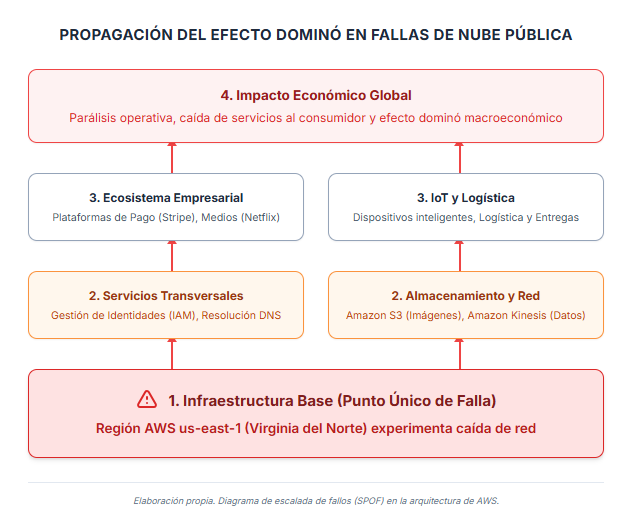
\includegraphics[width=0.85\textwidth]{diagrama.png}
\caption{Propagación del efecto dominó ante una interrupción en la infraestructura de AWS. Elaboración propia basada en AWS Post-Event Summaries.}
\label{fig:efecto_cascada}
\end{figure}

Estos acontecimientos demuestran que una alta disponibilidad contractual no elimina completamente la posibilidad de interrupciones masivas. Aunque AWS ofrece acuerdos de nivel de servicio (SLA) con porcentajes de disponibilidad muy elevados, la creciente dependencia mundial hacia un reducido número de proveedores incrementa el impacto potencial de cualquier incidente operativo. Por esta razón, numerosas organizaciones adoptan actualmente estrategias de redundancia, recuperación ante desastres y arquitecturas multi-nube con el objetivo de reducir los riesgos asociados a una dependencia excesiva de un único proveedor.\parencite{aws_network_2021}


\subsection{Debate Monopólico}
El crecimiento acelerado de la computación en la nube ha permitido optimizar el uso de los recursos tecnológicos y reducir la necesidad de que cada organización mantenga su propia infraestructura física. No obstante, el funcionamiento de centros de datos de gran escala también implica un elevado consumo de energía y recursos naturales. Debido a ello, el impacto ambiental de Amazon Web Services (AWS) se ha convertido en uno de los principales temas de discusión dentro de la industria tecnológica y en la comunidad científica.\parencite{climate_pledge_2019}

Los centros de datos de AWS operan de manera ininterrumpida para garantizar la disponibilidad de millones de aplicaciones alrededor del mundo. Esta operación requiere enormes cantidades de electricidad para alimentar servidores, dispositivos de almacenamiento, equipos de comunicación y sistemas de refrigeración. Como resultado, el consumo energético de la infraestructura cloud aumenta constantemente a medida que crece la demanda de servicios digitales, especialmente aquellos relacionados con la Inteligencia Artificial Generativa y el procesamiento masivo de datos.\parencite{climate_pledge_2019}

Con el objetivo de reducir este impacto, Amazon impulsa diversas iniciativas enfocadas en la sostenibilidad. Entre ellas destaca su participación en \textit{The Climate Pledge}, compromiso mediante el cual la empresa busca alcanzar emisiones netas de carbono iguales a cero antes del año 2040. Asimismo, AWS ha incrementado significativamente sus inversiones en proyectos de energía eólica y solar, convirtiéndose en uno de los mayores compradores corporativos de energía renovable a nivel mundial.\parencite{climate_pledge_2019}

Otra estrategia importante consiste en el desarrollo de hardware propio. Los procesadores AWS Graviton, diseñados por la propia compañía, ofrecen una mejor relación entre rendimiento y consumo energético en comparación con arquitecturas tradicionales. Esta optimización permite ejecutar una mayor cantidad de cargas de trabajo utilizando menos electricidad, mejorando la eficiencia global de los centros de datos.

Sin embargo, diversos investigadores señalan que la mejora en la eficiencia energética no elimina completamente el impacto ambiental. El aumento constante de usuarios y servicios hace que el consumo total continúe creciendo, fenómeno conocido como la Paradoja de Jevons, según la cual una tecnología más eficiente puede terminar incrementando el consumo total del recurso debido a su mayor utilización.\parencite{alcott2005jevons}

Además del consumo eléctrico, existen otros desafíos ambientales asociados a la infraestructura cloud. Uno de ellos corresponde al elevado uso de agua en los sistemas de refrigeración de algunos centros de datos, especialmente en regiones con escasez hídrica. Otro problema importante es la generación de residuos electrónicos, originados por la renovación periódica de servidores, discos de almacenamiento y otros componentes de hardware utilizados en la operación de la nube.

La Tabla \ref{tab:impacto_ambiental} resume los principales impactos ambientales asociados a AWS, las estrategias implementadas por la compañía y los desafíos que aún permanecen para la industria.

\begin{table}[H]
\centering
\renewcommand{\arraystretch}{1.5}
\caption{Impacto ambiental de AWS y principales desafíos de sostenibilidad}
\label{tab:impacto_ambiental}
\begin{tabular}{>{\centering\arraybackslash}p{3cm} p{5cm} p{4.5cm} p{3.5cm}}
\toprule
\textbf{Vector de Impacto} &
\textbf{Descripción del Riesgo} &
\textbf{Estrategia de Mitigación (AWS)} &
\textbf{Desafío Pendiente} \\
\midrule

\textbf{Consumo Energético} &
Elevada demanda de electricidad para servidores y sistemas de refrigeración. &
Uso creciente de energías renovables y procesadores Graviton de alta eficiencia. &
La mayor eficiencia también incrementa la demanda total de infraestructura (Paradoja de Jevons). \\

\textbf{Consumo de Agua} &
Uso intensivo de agua para refrigeración de centros de datos. &
Programas de gestión hídrica y proyectos Water Positive. &
Disponibilidad limitada de agua en regiones afectadas por sequías. \\

\textbf{Residuos Electrónicos} &
Renovación periódica de servidores y dispositivos tecnológicos. &
Reutilización de equipos y programas de reciclaje de componentes. &
Incremento continuo del volumen de residuos electrónicos a nivel mundial. \\

\bottomrule
\end{tabular}
\end{table}

En conjunto, estas iniciativas demuestran el compromiso de AWS por reducir el impacto ambiental de sus operaciones. Sin embargo, el crecimiento constante de la computación en la nube plantea nuevos desafíos relacionados con el consumo de recursos naturales y la sostenibilidad a largo plazo. En consecuencia, la eficiencia tecnológica deberá complementarse con políticas ambientales y modelos de operación que permitan equilibrar el desarrollo digital con la protección del medio ambiente.\parencite{climate_pledge_2019,alcott2005jevons}


\subsection{Perspectivas Regulatorias}
El crecimiento de Amazon Web Services (AWS) y de los principales proveedores de computación en la nube ha despertado un creciente interés por parte de los organismos reguladores de distintos países. A medida que una parte importante de la infraestructura digital mundial depende de un número reducido de empresas, los gobiernos han comenzado a analizar si las actuales condiciones del mercado favorecen realmente la competencia o, por el contrario, generan barreras que dificultan la entrada de nuevos participantes.\parencite{cma2025,eu_data_act_2023,eu_dma_2022}

Las principales preocupaciones regulatorias se centran en aspectos como la dependencia tecnológica de un único proveedor (\textit{vendor lock-in}), las tarifas de salida de datos (\textit{egress fees}), la falta de interoperabilidad entre plataformas y la creciente concentración del mercado en manos de AWS, Microsoft Azure y Google Cloud. Estas condiciones podrían limitar la capacidad de las organizaciones para migrar libremente entre proveedores y reducir la competencia dentro del sector.\parencite{cma2025}

Ante este escenario, diversas autoridades internacionales han iniciado investigaciones y desarrollado nuevas propuestas regulatorias para garantizar un mercado más competitivo y transparente. Entre las iniciativas más importantes destacan las siguientes:

\begin{itemize}

\item \textbf{Competition and Markets Authority (Reino Unido).} La CMA realizó una investigación sobre el mercado de servicios en la nube, concluyendo que existen prácticas comerciales que dificultan el cambio de proveedor, especialmente debido a las tarifas de salida de datos y a los descuentos condicionados por contratos de largo plazo. Como resultado, recomendó establecer medidas que promuevan una mayor competencia entre los proveedores de infraestructura cloud.\parencite{cma2025}

\item \textbf{Federal Trade Commission (Estados Unidos).} La FTC inició investigaciones relacionadas con las inversiones y alianzas estratégicas entre los principales proveedores de infraestructura cloud y las empresas dedicadas al desarrollo de Inteligencia Artificial Generativa. El objetivo es determinar si estas asociaciones podrían fortalecer aún más el poder de mercado de unas pocas compañías tecnológicas.\parencite{ftc_ai_2024}

\item \textbf{Unión Europea.} La Unión Europea ha impulsado diversas normas orientadas a facilitar la portabilidad de datos, mejorar la interoperabilidad entre plataformas y reducir las barreras para cambiar de proveedor. Entre las más relevantes se encuentran la \textit{Data Act} y la \textit{Digital Markets Act (DMA)}, las cuales buscan fortalecer la competencia y otorgar un mayor control de los datos a empresas y usuarios.\parencite{eu_data_act_2023,eu_dma_2022}

\end{itemize}

En paralelo, diferentes iniciativas internacionales promueven el desarrollo de arquitecturas abiertas y estrategias multi-nube, permitiendo que las organizaciones distribuyan sus servicios entre varios proveedores para reducir riesgos de dependencia y aumentar la resiliencia de sus sistemas.

En consecuencia, el futuro de la computación en la nube no dependerá únicamente de la innovación tecnológica, sino también del equilibrio entre competitividad, regulación y protección de los usuarios. Las políticas que actualmente se encuentran en desarrollo buscan garantizar que la infraestructura digital continúe creciendo bajo principios de transparencia, interoperabilidad y libre competencia, favoreciendo tanto a las empresas como a los consumidores finales.\parencite{cma2025,eu_data_act_2023,eu_dma_2022}
\newpage
\section{Conclusiones}
\newpage

\section{Referencias Bibliográficas}
\nocite{*} % <--- ESTA LÍNEA OBLIGA A MOSTRAR TODO LO QUE HAYA EN EL .BIB
\printbibliography[heading=none]
\newpage

\end{document}